% ---------------------------------------------------------------------------- %
\subsection{Produktumfeld}
% ---------------------------------------------------------------------------- %

%\textsc{TODO}

Das   Projekt   kann  grob   in   vier   Teilgebiete  unterteilt   werden: Die
Spannungsmessung, die Daten\"ubertragung, die Datenauswertung und die Speisung
des Sensors bzw. der Zentrale.


% ---------------------------------------------------------------------------- %
\subsection{Produkteigenschaften}
% ---------------------------------------------------------------------------- %

Unser  Produkt  dient  zur  \"Uberwachung der  Spannung  an  Solarmodulen. Die
gemessene  Spannung  wird \"uber  die  DC  Leitung  der Solaranlage  zu  einem
Masterger\"at  \"ubertragen,  welcher  die gemessenen  Werte  verarbeitet  und
allf\"allige  Fehler erkennt. Tritt  ein Fehler  auf, wird  eine entsprechende
Meldung  auf einem  Display  angezeigt, ein  Relais  f\"ur eine  zus\"atzliche
Alarmierung bet\"atigt und eine  Nachricht mittels SMS versendet. Dadurch wird
sichergestellt, dass defekte Solarmodule m\"oglichst schnell erkannt werden.

Die Bedienung des  Produktes wird einfach gehalten. Mittels  Touch Display auf
dem Masterger\"at k\"onnen die  n\"otigen Grundeinstellungen get\"atigt werden
und im  Fehlerfall wird die  Bezeichung des fehlerhaften  Moduls angezeigt. Im
Normalbetrieb muss keine Bedienung erfolgen.

\textsc{TODO}: Funktionen, Einsatz im Feld, Bedienungskonzept


% ---------------------------------------------------------------------------- %
\subsection{Systembereich}
% ---------------------------------------------------------------------------- %

Das System  besteht grunds\"atzlich  auf zwei Teilsysteme. Einerseits  aus der
Sensorplatine, welche in der Modulanschlussbox platziert ist, andererseits aus
dem Masterger\"at, welches beim Generatoranschlusskasten installiert ist.

Die Sensorplatine ist nur f\"ur die Datenerfassung zust\"andig.

%\textsc{TODO}: Noch ein wenig ausformulieren.
\begin{figure}[h!]
    \centering
    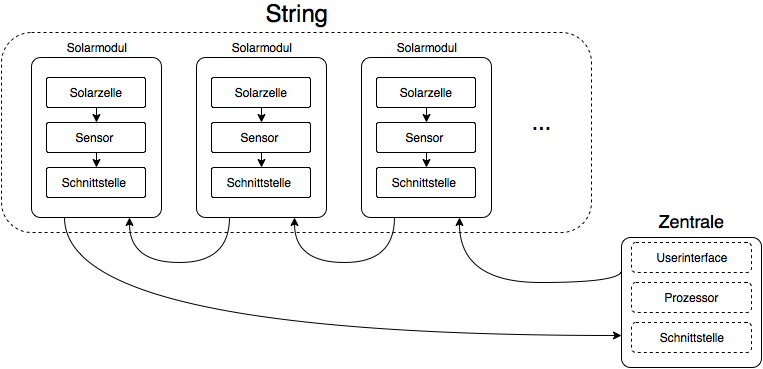
\includegraphics[width=.9\textwidth]{images/blockdiag.png}
    \caption{Blockdiagramm Hardwareaufbau}
    \label{fig:blockdiag:hardware}
\end{figure}


% TODO
% ---------------------------------------------------------------------------- %
\subsection{L\"osungsvarianten}
% ---------------------------------------------------------------------------- %
\textsc{TODO: am 07.04.2016 im Plenum}

% TODO
% ---------------------------------------------------------------------------- %
%\subsection{Evaluation L\"osungsvarianten}
% ---------------------------------------------------------------------------- %
%\textsc{TODO}
